\chapter{Quantum Machine Learning}
\label{cap:quantum_machine_learning}

Il Quantum Machine Learning (QML) rappresenta uno dei settori emergenti più promettenti nell'ambito del calcolo quantistico e dell'intelligenza artificiale, posizionandosi all'intersezione tra la meccanica quantistica e la teoria dell'apprendimento automatico\footnote{Biamonte, J., Wittek, P., Pancotti, N., Rebentrost, P., Wiebe, N., \& Lloyd, S. (2017). Quantum machine learning. \textit{Nature}, 549(7671), 195-202.}. Mentre i modelli classici analizzati nel Capitolo~\ref{cap:fondamenti_ml_classificazione_classica} elaborano l'informazione mediante strutture logiche deterministiche o probabilistiche tradizionali, il QML impiega lo spazio degli stati quantistici per rappresentare, trasformare e classificare dati complessi.

L'obiettivo di questo capitolo è definire il quadro teorico, matematico e architetturale della computazione quantistica applicata al machine learning, ponendo un accento specifico sui modelli di classificazione implementati nel framework Qiskit\footnote{Qiskit contributors. (2019). \textit{Qiskit: An Open-Source Framework for Quantum Computing}. Zenodo. \url{https://doi.org/10.5281/zenodo.2562110}. Per la voce BibTeX ufficiale si veda anche \url{https://github.com/Qiskit/qiskit/blob/main/CITATION.bib}.}. Nello specifico, verranno formalizzati i concetti di qubit, porte e circuiti quantistici parametrizzati; le strategie di mappatura dei dati classici in stati quantistici (\textit{data encoding}); le architetture di classificazione fondate sia sui metodi kernel quantistici (Quantum Support Vector Classifier, QSVC) sia sui modelli variazionali (Variational Quantum Classifier, VQC); ed infine un'analisi dettagliata dei limiti legati al rumore hardware e ai problemi di ottimizzazione.

\section{Fondamenti di Computazione Quantistica per l'Apprendimento Automatico}
\label{sec:fondamenti_computazione_quantistica}

A differenza dell'informatica classica basata sul bit binario $b \in \{0, 1\}$, la computazione quantistica sfrutta le proprietà vettoriali di sistemi fisici microscopici per codificare ed elaborare l'informazione in uno spazio di Hilbert complesso.

\subsection{Il Qubit e la Sfera di Bloch}
L'unità fondamentale dell'informazione nel calcolo quantistico è il \textit{qubit}. A differenza del bit classico, che può essere solo 0 o 1, un qubit sfrutta la meccanica quantistica per trovarsi in uno stato di sovrapposizione, rappresentando contemporaneamente sia lo 0 che l'1 con determinate probabilità. Un qubit è un sistema quantistico a due livelli, formalizzato come un vettore di stato unitario nello spazio di Hilbert complesso bidimensionale $\mathcal{H} \cong \mathbb{C}^2$. La base ortonormale canonica (o base computazionale) è definita dai due stati puri:
\begin{equation}
\ket{0} = \begin{pmatrix} 1 \\ 0 \end{pmatrix}, \quad \ket{1} = \begin{pmatrix} 0 \\ 1 \end{pmatrix},
\end{equation}
utilizzando la notazione bra-ket di Dirac. Sfruttando il principio di sovrapposizione, uno stato quantistico arbitrario $\ket{\psi}$ si esprime come combinazione lineare della base computazionale:
\begin{equation}
\ket{\psi} = \alpha \ket{0} + \beta \ket{1} = \begin{pmatrix} \alpha \\ \beta \end{pmatrix}, \quad \alpha, \beta \in \mathbb{C},
\end{equation}
con la condizione di normalizzazione imponendo che la probabilità totale sia unitaria:
\begin{equation}
|\alpha|^2 + |\beta|^2 = 1.
\end{equation}
In accordo con l'interpretazione di Born, $|\alpha|^2$ e $|\beta|^2$ rappresentano rispettivamente le probabilità di misurare lo stato $\ket{0}$ o $\ket{1}$ lungo la base computazionale.

A meno di una fase globale priva di significato fisico osservabile ($e^{i\gamma}$), qualsiasi stato puro di un singolo qubit può essere parametrizzato da due angoli reali $\theta \in [0, \pi]$ e $\phi \in [0, 2\pi)$:
\begin{equation}
\ket{\psi} = \cos\left(\frac{\theta}{2}\right)\ket{0} + e^{i\phi}\sin\left(\frac{\theta}{2}\right)\ket{1}.
\end{equation}
Questa formulazione fornisce una rappresentazione geometrica intuitiva nota come \textbf{Sfera di Bloch}, in cui ogni stato puro corrisponde a un punto identificato dal vettore unitario $(\sin\theta\cos\phi, \sin\theta\sin\phi, \cos\theta)^T$ sulla superficie della sfera di raggio unitario in $\mathbb{R}^3$.

Per un sistema composto da $n$ qubit, lo spazio di Hilbert globale è dato dal prodotto tensoriale degli spazi individuali $\mathcal{H}^{\otimes n} = \mathcal{H}_1 \otimes \mathcal{H}_2 \otimes \dots \otimes \mathcal{H}_n$, generato da $2^n$ stati di base ortonormali:
\begin{equation}
\ket{\psi} = \sum_{x \in \{0, 1\}^n} c_x \ket{x}, \quad \text{con } \sum_{x \in \{0, 1\}^n} |c_x|^2 = 1,
\end{equation}
dove $c_x \in \mathbb{C}$. La dimensione dello spazio degli stati cresce esponenzialmente con $n$, fornendo la base teorica per la potenziale capacità espressiva dei modelli quantistici rispetto al corrispondente spazio delle feature classico.

\begin{figure}[htbp]
    \centering
    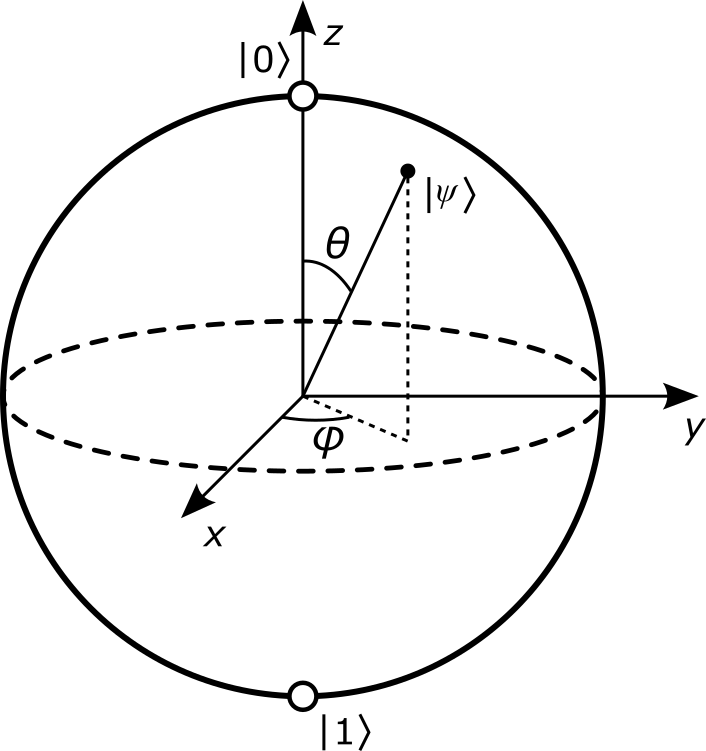
\includegraphics[width=0.35\textwidth]{assets/bloch_sphere.png}
    \caption{\footnotesize Rappresentazione geometrica di uno stato di un singolo qubit $\ket{\psi}$ sulla Sfera di Bloch parametrizzato dagli angoli polarizzazione $\theta$ e $\phi$. (Crediti: Di Smite-Meister - Opera propria, CC BY-SA 3.0, \url{https://commons.wikimedia.org/w/index.php?curid=5829358}).}
    \label{fig:bloch_sphere}
\end{figure}

\subsection{Operatori e Porte Logiche Quantistiche}
L'evoluzione temporale di un sistema quantistico chiuso è determinata dall'equazione di Schrödinger ed è modellata matematicamente da trasformazioni unitarie. Un operatore $U$ che agisce su $\mathcal{H}^{\otimes n}$ è unitario se soddisfa la condizione:
\begin{equation}
U^\dagger U = U U^\dagger = I,
\end{equation}
dove $U^\dagger$ denota l'operatore aggiunto Hermitiano (trasposto coniugato) di $U$ e $I$ è la matrice identità. La proprietà di unitarietà garantisce la conservazione della norma dello stato e quindi della probabilità totale.

Le trasformazioni elementari applicate ai registri di qubit prendono il nome di \textit{porte logiche quantistiche}. Tra le porte fondamentali a singolo qubit si annoverano le matrici di Pauli ($\sigma_x, \sigma_y, \sigma_z$), la porta di Hadamard ($H$) e le porte di rotazione parametrizzate ($R_x, R_y, R_z$):

\begin{itemize}
    \item \textbf{Matrici di Pauli:}
    \begin{equation}
    X = \begin{pmatrix} 0 & 1 \\ 1 & 0 \end{pmatrix}, \quad
    Y = \begin{pmatrix} 0 & -i \\ i & 0 \end{pmatrix}, \quad
    Z = \begin{pmatrix} 1 & 0 \\ 0 & -1 \end{pmatrix}.
    \end{equation}
    \item \textbf{Porta di Hadamard:} Genera uno stato di equa sovrapposizione partendo dai vettori della base computazionale:
    \begin{equation}
    H = \frac{1}{\sqrt{2}}\begin{pmatrix} 1 & 1 \\ 1 & -1 \end{pmatrix}, \quad H\ket{0} = \ket{+} = \frac{\ket{0}+\ket{1}}{\sqrt{2}}.
    \end{equation}
    \item \textbf{Porte di Rotazione Parametrizzate:} Definite tramite la funzione esponenziale di matrice $R_v(\theta) = \exp\left(-i \frac{\theta}{2} v\right)$ per $v \in \{X, Y, Z\}$:
    % \begin{equation}
    % R_x(\theta) = \begin{pmatrix} \cos\frac{\theta}{2} & -i\sin\frac{\theta}{2} \\ -i\sin\frac{\theta}{2} & \cos\frac{\theta}{2} \end{pmatrix}, \quad
    % R_y(\theta) = \begin{pmatrix} \cos\frac{\theta}{2} & -\sin\frac{\theta}{2} \\ \sin\frac{\theta}{2} & \cos\frac{\theta}{2} \end{pmatrix}, \quad
    % R_z(\theta) = \begin{pmatrix} e^{-i\frac{\theta}{2}} & 0 \\ 0 & e^{i\frac{\theta}{2}} \end{pmatrix}.
    % \end{equation}
    \begin{align}
    R_x(\theta) &= \begin{pmatrix} \cos\frac{\theta}{2} & -i\sin\frac{\theta}{2} \\ -i\sin\frac{\theta}{2} & \cos\frac{\theta}{2} \end{pmatrix}, \quad
    R_y(\theta) = \begin{pmatrix} \cos\frac{\theta}{2} & -\sin\frac{\theta}{2} \\ \sin\frac{\theta}{2} & \cos\frac{\theta}{2} \end{pmatrix}, \\
    R_z(\theta) &= \begin{pmatrix} e^{-i\frac{\theta}{2}} & 0 \\ 0 & e^{i\frac{\theta}{2}} \end{pmatrix}.
    \end{align}
\end{itemize}

L'interazione tra più qubit necessita di porte multi-qubit in grado di generare correlazioni non classiche. La porta a due qubit di riferimento è la porta \textbf{Controlled-NOT (CNOT)}, la quale inverte lo stato del qubit di target se e solo se il qubit di controllo si trova nel livello $\ket{1}$:
\begin{equation}
\text{CNOT} = \begin{pmatrix}
1 & 0 & 0 & 0 \\
0 & 1 & 0 & 0 \\
0 & 0 & 0 & 1 \\
0 & 0 & 1 & 0
\end{pmatrix}.
\end{equation}

\subsection{Entanglement e Sovrapposizione}
Mentre la sovrapposizione consente ad un singolo qubit di esistere come combinazione di più stati, l'\textbf{entanglement} è un fenomeno puramente quantistico privo di analogo classico. Seguendo la formalizzazione di Nielsen e Chuang\footnote{Nielsen, M. A., \& Chuang, I. L. (2010). \textit{Quantum Computation and Quantum Information}. Cambridge University Press.}, uno stato composito $\ket{\psi}_{AB} \in \mathcal{H}_A \otimes \mathcal{H}_B$ è definito \textit{entangled} se non può essere fattorizzato come prodotto tensoriale di stati singoli dei singoli sottosistemi:
\begin{equation}
\ket{\psi}_{AB} \neq \ket{\phi}_A \otimes \ket{\chi}_B.
\end{equation}

Un esempio classico di stato massimamente entangled è espresso dai quattro stati di Bell, tra cui:
\begin{equation}
\ket{\Phi^+} = \frac{1}{\sqrt{2}}(\ket{00} + \ket{11}) = \text{CNOT} (H \otimes I) \ket{00}.
\end{equation}
Nei modelli di QML, l'entanglement gioca un ruolo cruciale: consente l'elaborazione simultanea delle correlazioni tra le feature del dataset classico, permettendo al modello quantistico di estrarre pattern complessi e non-locali che richiederebbero approssimazioni computazionalmente onerose in contesti classici.

\begin{figure}[htbp]
    \centering
    \begin{quantikz}
    \lstick{$\ket{0}$} & \gate{H} & \ctrl{1} & \qw \\
    \lstick{$\ket{0}$} & \qw      & \targ{}  & \qw
    \end{quantikz}
    \quad
    $\Bigg\}\dfrac{\ket{00}+\ket{11}}{\sqrt{2}}$
    \caption{\footnotesize Schema di un circuito quantistico elementare per la generazione dello stato entangled di Bell $\ket{\Phi^+}$ mediante l'applicazione in cascata di una porta Hadamard $H$ ed una porta CNOT.}
    \label{fig:bell_state_circuit}
\end{figure}

\subsection{Circuiti Quantistici Parametrizzati (PQC)}
I \textbf{Circuiti Quantistici Parametrizzati} (\textit{Parameterized Quantum Circuits}, PQC) costituiscono la base delle architetture di machine learning quantistico attuali (era NISQ)\footnote{Preskill, J. (2018). Quantum Computing in the NISQ era and beyond. \textit{Quantum}, 2, 79.}. Un PQC (noto anche come \textit{Ansatz}) è una sequenza di porte quantistiche di cui una parte è governata da un vettore di parametri reali ed ottimizzabili $\boldsymbol{\theta} \in \mathbb{R}^m$.

Matematicamente, la trasformazione globale operata dal circuito è descritta dal prodotto ordinato di $L$ operatori unitari:
\begin{equation}
U(\boldsymbol{\theta}) = U_L(\theta_L) U_{L-1}(\theta_{L-1}) \cdots U_1(\theta_1) = \prod_{l=1}^{L} U_l(\theta_l).
\end{equation}
Se l'operatore $U_l(\theta_l)$ deriva da un generatore Hermitiano $H_l$ (operatore distinto dallo spazio di Hilbert $\mathcal{H}$ e dalla porta di Hadamard $H$ introdotti in precedenza), la sua forma esplicita è $U_l(\theta_l) = \exp(-i \theta_l H_l)$. La flessibilità espressiva e l'architettura dei PQC influenzano direttamente la capacità di generalizzazione del modello quantistico e determinano l'efficienza della procedura di ottimizzazione dei parametri.

\section{Data Encoding e Mappatura delle Feature}
\label{sec:data_encoding}

Poiché gli algoritmi di calcolo quantistico operano esclusivamente su vettori di stato appartenenti ad uno spazio di Hilbert, una fase preliminare e fondamentale riguarda il \textbf{Data Encoding} (\textit{Quantum Feature Mapping}). Tale processo converte un vettore di feature classiche $\mathbf{x} = (x_1, x_2, \dots, x_d)^T \in \mathbb{R}^d$ in uno stato quantistico $\ket{\psi(\mathbf{x})} \in \mathcal{H}^{\otimes n}$ tramite una mappa non lineare $\Phi: \mathcal{X} \to \mathcal{H}$:
\begin{equation}
\ket{\psi(\mathbf{x})} = U_{\Phi}(\mathbf{x}) \ket{0}^{\otimes n},
\end{equation}
dove $U_{\Phi}(\mathbf{x})$ rappresenta l'operatore unitario di codifica.

La scelta della tecnica di encoding impatta direttamente sulla dimensionalità del circuito, sulla profondità necessaria per la preparazione dello stato e sulla natura delle relazioni matematiche che il modello sarà in grado di identificare.

\subsection{Tecniche di Codifica Fondamentali}

Si distinguono quattro principali strategie per l'encoding dei dati classici:

\begin{enumerate}
    \item \textbf{Basis Encoding:} Mappa un vettore binario classico $\mathbf{x} \in \{0, 1\}^d$ direttamente nel corrispondente stato della base computazionale $\ket{\mathbf{x}} = \ket{x_1 x_2 \cdots x_d}$. Questa tecnica richiede $n = d$ qubit ed è adatta per algoritmi di ricerca o elaborazione di strutture dati booleane, ma non sfrutta la continuità dello spazio degli stati quantistici.
    \item \textbf{Amplitude Encoding:} Mappa un vettore di dati reale e normalizzato $\mathbf{x} \in \mathbb{R}^d$ con $\|\mathbf{x}\|_2 = 1$ nelle ampiezze di probabilità di uno stato quantistico:
    \begin{equation}
    \ket{\psi(\mathbf{x})} = \sum_{i=1}^{d} x_i \ket{i-1},
    \end{equation}
    dove $d \le 2^n$. Il vantaggio risiede nell'efficienza spaziale: un registro di $n$ qubit può codificare un vettore di dimensione $d = 2^n$, offrendo una compressione esponenziale. Tuttavia, la preparazione dello stato $U_\Phi(\mathbf{x})$ richiede una complessità in termini di porte logiche pari a $O(2^n)$ nel caso generale, limitandone l'applicabilità pratica su hardware NISQ privi di QRAM (\textit{Quantum Random Access Memory})\footnote{Giovannetti, V., Lloyd, S., \& Maccone, L. (2008). Quantum random access memory. \textit{Physical Review Letters}, 100(16), 160501.}.
    \item \textbf{Angle Encoding:} Mappa ogni componente $x_i$ del vettore classico nell'angolo di rotazione di un singolo qubit. Per un vettore di dimensione $d$, si impiegano $n = d$ qubit applicando rotazioni parametrizzate:
    \begin{equation}
    \ket{\psi(\mathbf{x})} = \bigotimes_{i=1}^{d} R_v(x_i) \ket{0}, \quad v \in \{x, y, z\}.
    \end{equation}
    Questa tecnica presenta una profondità di circuito costante $O(1)$, ed è ampiamente utilizzata su hardware reali, a fronte di una scalabilità lineare nel numero di qubit $n = d$.
    \item \textbf{Flexible / Dense Angle Encoding:} Variante dell'Angle Encoding che consente di codificare due valori continui $(x_i, x_{i+1})$ su un singolo qubit sfruttando sia l'angolo di inclinazione $\theta$ sia la fase relativa $\phi$ della Sfera di Bloch:
    \begin{equation}
    \ket{\psi(x_i, x_{i+1})} = \cos(x_i)\ket{0} + e^{i x_{i+1}}\sin(x_i)\ket{1}.
    \end{equation}
\end{enumerate}

\subsection{Quantum Feature Maps Avanzate in Qiskit}
In Qiskit, la mappa di feature genera relazioni non lineari tra le componenti del vettore x combinando rotazioni sui singoli qubit e porte di entanglement.

L'operatore di mappatura è strutturato alternando strati trasversali di porte di Hadamard $H^{\otimes n}$ a strati di evoluzione diagonale $U_S(\mathbf{x})$, generati da prodotti di operatori di Pauli e responsabili sia dei termini di codifica a singolo qubit sia delle correlazioni (entangling) tra coppie o k-tuple di qubit:
\begin{equation}
U_{\Phi}(\mathbf{x}) = \left( U_S(\mathbf{x}) H^{\otimes n} \right)^r,
\end{equation}
dove $r$ indica il numero di ripetizioni del circuito (\textit{reps}). L'operatore unitario generico $U_S(\mathbf{x})$ si esprime come:
\begin{equation}
U_S(\mathbf{x}) = \exp\left( i \sum_{S \subseteq \{1, \dots, n\}} \phi_S(\mathbf{x}) \prod_{i \in S} P_i \right),
\end{equation}
dove $P_i \in \{I, X, Y, Z\}$ sono gli operatori di Pauli e $\phi_S(\mathbf{x})$ rappresenta una funzione reale scalare dipendente dalle componenti di $\mathbf{x}$.

\subsubsection{PauliFeatureMap}
Il \textbf{PauliFeatureMap} è un circuito di codifica dei dati del framework Qiskit e costituisce l'infrastruttura generale per la costruzione di feature map customizzate basate sull'algebra delle matrici di Pauli. Definito l'insieme delle stringhe di Pauli desiderate (es. $P = \{'X', 'Y', 'ZZ'\}$), la mappa genera un circuito quantistico che codifica sia termini lineari ($\phi_{\{i\}}(\mathbf{x}) = x_i$) sia correlazioni tra coppie o k-tuple di variabili.

\subsubsection{ZZFeatureMap}
La \textbf{ZZFeatureMap} è una variante della \texttt{PauliFeatureMap} progettata per codificare le interazioni di secondo ordine ($x_i \cdot x_j$) tra le componenti dei dati. Tali correlazioni non lineari generano uno spazio di feature quantistico complesso, la cui simulazione classica diventa computazionalmente intrattabile al crescere delle dimensioni del sistema \footnote{Havl{\'\i}{\v{e}}ck, V., Córcoles, A. D., Temme, K., Harrow, A. W., Kandala, A., Chow, J. M., \& Gambetta, J. M. (2019). Supervised learning with quantum-enhanced feature spaces. \textit{Nature}, 567(7747), 209-214.}.

Per una rete di $n$ qubit, la ZZFeatureMap definisce:
\begin{itemize}
    \item Interazioni a singolo qubit: $\phi_{\{i\}}(\mathbf{x}) = x_i$;
    \item Interazioni a due qubit: $\phi_{\{i, j\}}(\mathbf{x}) = (\pi - x_i)(\pi - x_j)$.
\end{itemize}

L'operatore unitario risultante per uno strato ha la seguente espressione analitica:
\begin{equation}
U_{\Phi_{\text{ZZ}}}(\mathbf{x}) = \prod_{i < j} e^{i (\pi - x_i)(\pi - x_j) Z_i Z_j} \bigotimes_{k=1}^n e^{i x_k Z_k} H^{\otimes n}.
\end{equation}
L'operatore $e^{i \phi Z_i Z_j}$ viene implementato sul circuito quantistico tramite una sequenza composta da una porta CNOT, una rotazione $R_z(2\phi)$ sul qubit target e un'ulteriore CNOT per ripristinare il corretto stato di entanglement.

% \begin{figure}[htbp]
%     \centering
%     % PLACEHOLDER FOTO: Circuito della ZZFeatureMap a 2 Qubit
%     %\includegraphics[width=0.65\textwidth]{assets/zz_feature_map_circuit.png}
%     \caption{\footnotesize Struttura del circuito quantistico per una $\text{ZZFeatureMap}$ su $n=2$ qubit con 1 ripetizione ($r=1$), evidenziante le rotazioni individuali $R_z(x_i)$ e la porta condizionata $ZZ$ per le interazioni incrociate.}
%     \label{fig:zz_feature_map_circuit}
% \end{figure}

\begin{figure}[ht]
    \centering
    \begin{quantikz}
        \lstick{$q_0$} & \gate{H} & \gate{R_z(x_0)} & \ctrl{1} & \gate{R_z(\phi(x_0,x_1))} & \ctrl{1} & \qw \\
        \lstick{$q_1$} & \gate{H} & \gate{R_z(x_1)} & \targ{}  & \gate{R_z(\phi(x_0,x_1))} & \targ{}  & \qw
    \end{quantikz}
    \caption{Circuito quantistico della \textit{ZZFeatureMap} per $n=2$ qubit
    e una ripetizione ($r=1$), con le rotazioni $R_z(x_i)$ per la codifica
    delle variabili e l'interazione a due qubit di tipo $ZZ$.}
    \label{fig:zz_feature_map_circuit}
\end{figure}

\section{Architetture di Classificazione Quantistica in Qiskit}
\label{sec:architetture_qiskit}

L'applicazione del calcolo quantistico ai problemi di classificazione supervisionata analizzati nel Capitolo~\ref{cap:fondamenti_ml_classificazione_classica} segue due paradigmi principali: il paradigma basato su kernel quantistici (\textbf{Quantum Support Vector Classifier}, QSVC) e il paradigma basato su circuiti variazionali (\textbf{Variational Quantum Classifier}, VQC).

\subsection{QSVC: Quantum Support Vector Classifier e Quantum Kernel Estimation}
Il paradigma QSVC estende la teoria delle Support Vector Machines esposta nella Sezione~\ref{sec:svm_classica} introducendo il concetto di \textbf{Quantum Kernel Estimation (QKE)}.

Come formalizzato per le SVM classiche, la formulazione duale di Wolfe richiede il calcolo del prodotto scalare tra le immagini trasformate dei dati $K(\mathbf{x}_i, \mathbf{x}_j) = \langle \Phi(\mathbf{x}_i), \Phi(\mathbf{x}_j) \rangle_{\mathcal{F}}$. Nel contesto quantistico, lo spazio delle feature $\mathcal{F}$ coincide con lo spazio di Hilbert $\mathcal{H}$, e la funzione kernel quantistica misura la sovrapposizione (o \textit{fedeltà}) tra due stati quantistici preparati a partire da due differenti campioni di input $\mathbf{x}_i$ e $\mathbf{x}_j$:
\begin{equation}
K_{\text{quantum}}(\mathbf{x}_i, \mathbf{x}_j) = \left| \braket{\psi(\mathbf{x}_i)}{\psi(\mathbf{x}_j)} \right|^2 = \left| \bra{0}^{\otimes n} U_{\Phi}^\dagger(\mathbf{x}_j) U_{\Phi}(\mathbf{x}_i) \ket{0}^{\otimes n} \right|^2.
\end{equation}

\subsubsection{FidelityQuantumKernel}
Nel framework Qiskit, il calcolo analitico o sperimentale della matrice di Gram quantistica è affidato alla classe \texttt{FidelityQuantumKernel}. Il processo operativo si articola nelle seguenti fasi:
\begin{enumerate}
    \item Preparazione dello stato iniziale $\ket{0}^{\otimes n}$.
    \item Applicazione dell'operatore di encoding $U_{\Phi}(\mathbf{x}_i)$ associato al primo campione.
    \item Applicazione dell'operatore aggiunto $U_{\Phi}^\dagger(\mathbf{x}_j)$ associato al secondo campione.
    \item Misurazione del registro nella base computazionale.
\end{enumerate}

La probabilità di osservare lo stato $\ket{0}^{\otimes n}$ al termine della misurazione (ovvero il rapporto tra il numero di conteggi della stringa interamente nulla e il totale degli \textit{shots} eseguiti $N_{\text{shots}}$) corrisponde esattamente alla fedeltà quantistica $K_{\text{quantum}}(\mathbf{x}_i, \mathbf{x}_j)$:
\begin{equation}
\hat{K}(\mathbf{x}_i, \mathbf{x}_j) = \frac{N_{\text{shots}}(\ket{0\dots0})}{N_{\text{shots}}}.
\end{equation}

Una volta costruita l'intera matrice di Kernel quantistica $\mathbf{K} \in \mathbb{R}^{N \times N}$, dove $N$ indica il numero di campioni del training set, essa viene passata a un solver di programmazione quadratica classico per risolvere il duale di Wolfe e determinare i moltiplicatori di Lagrange $\alpha_k$:
\begin{equation}
f(\mathbf{x}) = \text{sign}\left( \sum_{k \in \text{SV}} \alpha_k y_k K_{\text{quantum}}(\mathbf{x}_k, \mathbf{x}) + b \right).
\end{equation}

\begin{figure}[htbp]
    \centering
    \begin{tikzpicture}[
        node distance=1.1cm and 1.6cm,
        box/.style={draw, rounded corners, minimum height=1.1cm, minimum width=3.2cm,
                     align=center, fill=blue!5, font=\footnotesize},
        arrow/.style={-{Latex[length=2mm]}, thick}
    ]
        \node[box] (data) {Dati classici\\ $\mathbf{x}_i,\ \mathbf{x}_j$};
        \node[box, below=of data] (circuit) {Circuito quantistico\\ $U_{\Phi}(\mathbf{x}_i)\,U_{\Phi}^\dagger(\mathbf{x}_j)$};
        \node[box, below=of circuit] (fidelity) {Stimatore di fedelt\`a quantistica\\ $\left|\langle 0|U_{\Phi}^\dagger(\mathbf{x}_j)U_{\Phi}(\mathbf{x}_i)|0\rangle\right|^2$};
        \node[box, below=of fidelity] (gram) {Costruzione matrice di Gram\\ $K_{ij} = \text{Fedelt\`a}(\mathbf{x}_i,\mathbf{x}_j)$};
        \node[box, below=of gram] (opt) {Ottimizzazione convessa classica\\ (SVM su $K$)};
        \node[box, below=of opt] (hyperplane) {Iperpiano separatore};

        \draw[arrow] (data) -- (circuit);
        \draw[arrow] (circuit) -- (fidelity);
        \draw[arrow] (fidelity) -- (gram);
        \draw[arrow] (gram) -- (opt);
        \draw[arrow] (opt) -- (hyperplane);
    \end{tikzpicture}
    \caption{\footnotesize Schema concettuale dell'architettura QSVC: codifica dei dati tramite circuito $U_{\Phi}(\mathbf{x}_i) U_{\Phi}^\dagger(\mathbf{x}_j)$, stimatore di fedelt\`a quantistica, costruzione della matrice di Gram ed ottimizzazione convessa classica per la ricerca dell'iperpiano separatore.}
    \label{fig:qsvc_architecture_flow}
\end{figure}

\subsection{VQC: Variational Quantum Classifier}
Il \textbf{Variational Quantum Classifier (VQC)}\footnote{Mitarai, K., Negoro, M., Kitagawa, M., \& Fujii, K. (2018). Quantum circuit learning. \textit{Physical Review A}, 98(3), 032309.} è un modello di apprendimento quantistico-classico ibrido che implementa una rete neurale quantistica (\textit{Quantum Neural Network}, QNN). La struttura complessiva si fonda sull'interazione iterativa tra un processore quantistico (QPU) che valuta la funzione obiettivo e un ottimizzatore classico gestito dalla CPU.

Un'architettura VQC si compone di quattro moduli interconnessi:
\begin{enumerate}
    \item \textbf{Feature Map Circuit ($U_{\Phi}(\mathbf{x})$):} Mappa il vettore $x$ nello stato $\ket{\psi(\mathbf{x})}$.
    \item \textbf{Ansatz Variational Circuit ($W(\boldsymbol{\theta})$):} Circuiti quantistici parametrizzati le cui rotazioni sono controllate dal vettore $\boldsymbol{\theta}$.
    \item \textbf{Modulo di Misura e Post-processing:} Misura i qubit osservabili per ottenere valori di aspettazione o probabilità di classe.
    \item \textbf{Ottimizzatore Classico:} Aggiorna i parametri $\boldsymbol{\theta}$ minimizzando una loss function definita.
\end{enumerate}

Lo stato finale elaborato dal circuito prima della misura ha la forma:
\begin{equation}
\ket{\psi(\mathbf{x}, \boldsymbol{\theta})} = W(\boldsymbol{\theta}) U_{\Phi}(\mathbf{x}) \ket{0}^{\otimes n}.
\end{equation}

\begin{figure}[htbp]
    \centering
    \begin{tikzpicture}[
        node distance=2.4cm,
        box/.style={draw, rounded corners, minimum height=1.3cm, minimum width=3.6cm,
                     align=center, fill=blue!5, font=\footnotesize},
        arrow/.style={-{Latex[length=2mm]}, thick}
    ]
        \node[box] (quantum) {Circuito quantistico\\ $U(\boldsymbol{\theta})$\\ valutazione $\langle \hat{O} \rangle$};
        \node[box, right=of quantum] (classical) {Ottimizzatore classico\\ aggiornamento $\boldsymbol{\theta}$};

        \draw[arrow] (quantum.north) to[bend left=35] node[above, font=\scriptsize] {valore di aspettazione $\langle \hat{O} \rangle$} (classical.north);
        \draw[arrow] (classical.south) to[bend left=35] node[below, font=\scriptsize] {parametri aggiornati $\boldsymbol{\theta}$} (quantum.south);
    \end{tikzpicture}
    \caption{\footnotesize Architettura del ciclo ibrido di addestramento in un Variational Quantum Classifier (VQC). Il circuito quantistico valuta il valore di aspettazione dell'osservabile, mentre l'ottimizzatore classico calcola l'aggiornamento dei parametri $\boldsymbol{\theta}$.}
    \label{fig:vqc_hybrid_loop}
\end{figure}

\subsection{Struttura degli Ansatz Variabili}
L'Ansatz $W(\boldsymbol{\theta})$ definisce lo spazio degli stati raggiungibili dal circuito parametrico, influenzando direttamente l'espressività del modello e la trattabilità del processo di ottimizzazione classica dei parametri. Tra le famiglie di Ansatz più diffuse in Qiskit si annoverano:

\begin{itemize}
    \item \textbf{RealAmplitudes:} Costituito da strati alternati di rotazioni a singolo qubit attorno all'asse $Y$ ($R_y(\theta)$) e porte di entanglement non parametrizzate (tipicamente CNOT disposte secondo un pattern lineare, circolare o full). Poiché tutte le operazioni sono descritte da matrici a coefficienti reali, lo stato risultante è vincolato ad ampiezze appartenenti a $\mathbb{R}^{2^n}$, escludendo quindi la componente di fase complessa dello spazio di Hilbert.

    \item \textbf{EfficientSU2:} Estensione più espressiva che implementa rotazioni generiche del gruppo speciale unitario $SU(2)$, combinando porte $R_y$ e $R_z$ su ogni qubit e intervallandole con layer di entanglement. Questa struttura consente di esplorare l'intero spazio di Hilbert accessibile con $n$ qubit.

    \item \textbf{TwoLocal:} Ansatz generico e altamente personalizzabile, costruito alternando blocchi di porte a singolo qubit parametrizzate a blocchi di entanglement a due qubit, su una topologia di connessione configurabile dall'utente.
\end{itemize}

\begin{figure}[htbp]
    \centering

    \begin{subfigure}{\textwidth}
        \centering
        \begin{quantikz}
            \lstick{$q_0$} & \gate{R_y(\theta_0)} & \ctrl{1} & \gate{R_y(\theta_2)} & \qw \\
            \lstick{$q_1$} & \gate{R_y(\theta_1)} & \targ{}  & \gate{R_y(\theta_3)} & \qw
        \end{quantikz}
        \caption{RealAmplitudes}
        \label{fig:realamplitudes}
    \end{subfigure}

    \vspace{0.5cm}

    \begin{subfigure}{\textwidth}
        \centering
        \begin{quantikz}
            \lstick{$q_0$} & \gate{R_y(\theta_0)} & \gate{R_z(\theta_2)} & \ctrl{1} & \gate{R_y(\theta_4)} & \gate{R_z(\theta_6)} & \qw \\
            \lstick{$q_1$} & \gate{R_y(\theta_1)} & \gate{R_z(\theta_3)} & \targ{}  & \gate{R_y(\theta_5)} & \gate{R_z(\theta_7)} & \qw
        \end{quantikz}
        \caption{EfficientSU2}
        \label{fig:efficientsu2}
    \end{subfigure}

    \caption{\footnotesize Diagramma della struttura di porte per le architetture Ansatz $\text{RealAmplitudes}$ ed $\text{EfficientSU2}$ a due qubit con ripetizione $r=1$ (TwoLocal, essendo configurabile arbitrariamente, non è illustrato graficamente in quanto le due architetture precedenti ne rappresentano casi particolari).}
    \label{fig:ansatz_comparison}
\end{figure}

\subsection{Funzioni di Costo e Tecniche di Calcolo del Gradiente}
Per un problema di classificazione binaria con etichette $y_i \in \{0, 1\}$, la predizione del VQC può essere estratta definendo un osservabile Hermitiano $M$ (es. $M = Z_0$, l'operatore di Pauli-Z applicato al primo qubit). Il valore atteso dell'osservabile è fornito da:
\begin{equation}
\langle M \rangle_{\mathbf{x}, \boldsymbol{\theta}} = \bra{\psi(\mathbf{x}, \boldsymbol{\theta})} M \ket{\psi(\mathbf{x}, \boldsymbol{\theta})}.
\end{equation}
Tale valore atteso, compreso nell'intervallo $[-1, 1]$, viene trasformato in una probabilità di classe $\hat{p} \in [0, 1]$ mediante una mappatura affine $\hat{p}_i = \frac{\langle M \rangle + 1}{2}$.

L'addestramento del VQC richiede la minimizzazione della perdita empirica regolarizzata:
\begin{equation}
\mathcal{L}(\boldsymbol{\theta}) = \frac{1}{n} \sum_{i=1}^{n} L_{\text{ce}}(y_i, \hat{p}_i(\mathbf{x}_i, \boldsymbol{\theta})),
\end{equation}
dove $L_{\text{ce}}$ rappresenta la Binary Cross-Entropy formalizzata nel Capitolo~\ref{cap:fondamenti_ml_classificazione_classica}.

Per applicare algoritmi di ottimizzazione basati su gradiente (es. Gradient Descent, Adam) direttamente su un computer quantistico hardware o un emulatore, la derivata parziale della funzione di costo rispetto al parametro $\theta_k$ viene valutata analiticamente senza approssimazioni alle differenze finite mediante la \textbf{Parameter-Shift Rule}\footnote{Schuld, M., Bergholm, V., Gogolin, C., Izaac, J., \& Killoran, N. (2019). Evaluating analytic gradients on quantum hardware. \textit{Physical Review A}, 99(3), 032331.}:
\begin{equation}
\frac{\partial \langle M \rangle}{\partial \theta_k} = r \left( \langle M \rangle_{\theta_k + s} - \langle M \rangle_{\theta_k - s} \right),
\end{equation}
dove per porte di rotazione generate da generatori con autovalori $\pm \frac{1}{2}$ (es. porte di Pauli), il moltiplicatore scalare è $r = \frac{1}{2}$ e lo shift angolare è $s = \frac{\pi}{2}$.

\subsection{Ottimizzatori Classici per Architetture Variazionali}
L'ottimizzazione dei parametri $\boldsymbol{\theta}$ in presenza di rumore hardware o fluttuazioni stocastiche nella stima delle ampiezze richiede la scelta di ottimizzatori dedicati:

\begin{itemize}
    \item \textbf{COBYLA (Constrained Optimization BY Linear Approximation):} Algoritmo privo di derivate che modella la funzione obiettivo con approssimazioni lineari su un simplesso. Estremamente robusto a modesti livelli di rumore di shot.
    \item \textbf{SPSA (Simultaneous Perturbation Stochastic Approximation):} Algoritmo stocastico ad alto rendimento, progettato per contesti ad alta varianza. Approssima il gradiente dell'intera funzione di costo valutando soltanto due misurazioni quantistiche per iterazione, indipendentemente dalla dimensione del vettore dei parametri $m$, perturbando simultaneamente tutti i $\theta_k$.
    \item \textbf{L-BFGS (Limited-memory BFGS) / SLSQP (Sequential Least Squares Programming):} Algoritmi deterministici di tipo Quasi-Newton e programmazione quadratica sequenziale, ampiamente impiegati in contesti simulati esenti da rumore stocastico (\textit{statevector simulation}).
\end{itemize}

\subsection{Confronto Analitico ed Architetturale: QSVC vs VQC}
La scelta tra un approccio basato su kernel quantistici (QSVC) ed un approccio variazionale (VQC) implica precisi bilanciamenti dal punto di vista metodologico e computazionale, sintetizzati nella Tabella~\ref{tab:confronto_qsvc_vqc}.

\begin{table}[htbp]
\centering
\caption{Confronto architetturale e metodologico tra i modelli QSVC e VQC.}
\label{tab:confronto_qsvc_vqc}
\small
\renewcommand{\arraystretch}{1.2}
\begin{tabularx}{\textwidth}{l|X|X}
\hline
\textbf{Proprietà} & \textbf{QSVC (Quantum Kernel)} & \textbf{VQC (Variational Circuit)} \\
\hline
\textbf{Paradigma} & Kernel Method (Programmazione Quadratica Convessa). & Rete Neurale Quantistica (Ottimizzazione Non-Convessa Ibrida). \\
\textbf{Ottimizzazione} & Convessa con minimo globale unico e ben definito. & Non-convessa, soggetta a minimi locali e Barren Plateaus. \\
\textbf{Fase di Training} & $O(N^2)$ valutazioni del kernel quantistico per $N$ campioni. & Dipendente da (N. iterazioni $\times$ N. campioni $\times$ N. parametri). \\
\textbf{Sensibilità al Rumore} & Sensibile all'accumulo di rumore nella matrice di Gram. & Inerentemente più tollerante al rumore (\textit{error mitigation} naturale). \\
\textbf{Parametri Modello} & Moltiplicatori di Lagrange $\alpha_i$ associati ai campioni. & Vettore di angoli del PQC $\boldsymbol{\theta}$ di dimensione fissa. \\
\hline
\end{tabularx}
\end{table}

\section{Complessità Computazionale, Sfide Metodologiche e Limiti Hardware}
\label{sec:sfide_e_limiti}

Sebbene i modelli di Quantum Machine Learning offrano teoricamente l'accesso a spazi di rappresentazione ad elevata dimensionalità, l'applicazione pratica su hardware reali attuali risente di rilevanti vincoli teorici e fisici.

\subsection{Analisi della Complessità Computazionale e di Spazio}
La complessità di esecuzione di un algoritmo QML è determinata da tre risorse fondamentali:
\begin{enumerate}
    \item \textbf{Numero di Qubit ($n$):} Vincolato alla dimensione del vettore delle feature $d$ (o a $\log_2 d$ nel caso di Amplitude Encoding).
    \item \textbf{Profondità del Circuito ($D$):} Il numero massimo di porte quantistiche lungo il percorso critico del circuito. La profondità condiziona direttamente il tempo di coerenza richiesto.
    \item \textbf{Shot Noise e Varianza di Campionamento:} La stima del valore atteso di un osservabile con incertezza $\epsilon$ richiede un numero di misurazioni ($shots$) pari a:
    \begin{equation}
    N_{\text{shots}} = O\left(\frac{1}{\epsilon^2}\right),
    \end{equation}
    in accordo con il Teorema del Limite Centrale.
\end{enumerate}

Per l'architettura QSVC, la costruzione della matrice di Gram richiede il calcolo di $\frac{N(N-1)}{2}$ elementi distinti, dove $N$ è il numero di campioni del training set (da non confondere con il numero di qubit $n$ impiegati dal circuito di encoding). Ciascun elemento necessita di un circuito di profondità $2 D_{\Phi}$ seguito da $N_{\text{shots}}$ valutazioni. Per il VQC, la complessità di ciascuna epoca di training è scalata dal numero di parametri $m$ moltiplicato per il costo di calcolo del gradiente ($2m$ valutazioni quantistiche per passo usando la Parameter-Shift Rule).

\subsection{Il Fenomeno dei Barren Plateaus}
Un ostacolo fondamentale nell'addestramento dei circuiti quantistici variazionali è il fenomeno dei \textbf{Barren Plateaus} (altipiani sterili)\footnote{McClean, J. R., Boixo, S., Smelyanskiy, V. N., Babbush, R., \& Neven, H. (2018). Barren plateaus in quantum neural network training landscapes. \textit{Nature Communications}, 9(1), 4812.}.

Quando un PQC mostra un livello elevato di espressività e l'Ansatz forma un $2$-design di Haar sullo spazio di Hilbert, la varianza delle derivate parziali della funzione di costo decresce esponenzialmente al crescere del numero di qubit $n$:
\begin{equation}
\text{Var}_{\boldsymbol{\theta}} \left[ \frac{\partial \mathcal{L}(\boldsymbol{\theta})}{\partial \theta_k} \right] \in O\left( \frac{1}{2^n} \right).
\end{equation}

Questo implica che il paesaggio della funzione di costo (\textit{loss landscape}) diventa esponenzialmente piatto sulla quasi totalità dello spazio dei parametri, rendendo i gradienti numericamente impercettibili per gli ottimizzatori classici in presenza di rumore stocastico o di campionamento. Le strategie per mitigare questo fenomeno comprendono l'adozione di Ansatz locali, la pre-inizializzazione mirata dei parametri, o la progettazione di architetture strutturate ispirate alle simmetrie del problema (\textit{Equivariant Quantum Neural Networks}).

\begin{figure}[htbp]
    \centering
    \begin{tikzpicture}
        \begin{axis}[
            width=0.72\textwidth,
            height=5.5cm,
            axis lines=middle,
            xlabel={$\theta_k$},
            ylabel={$\mathcal{L}(\boldsymbol{\theta})$},
            xtick=\empty,
            ytick=\empty,
            xmin=-3, xmax=3,
            ymin=-0.15, ymax=1.3,
            domain=-3:3,
            samples=300,
            smooth,
            thick,
            clip=false,
        ]
            \addplot[color=blue!70!black, thick] {1 - exp(-x^2/0.01)};

            % Annotazione: regione piatta (barren plateau)
            \draw[-{Latex[length=2mm]}] (axis cs:-2,1.05) -- (axis cs:-1,1.0);
            \node[align=center, font=\footnotesize] at (axis cs:-2,1.15) {Regione piatta\\(gradiente $\approx 0$)};

            % Annotazione: narrow gorge
            \draw[-{Latex[length=2mm]}] (axis cs:1.2,0.5) -- (axis cs:0.15,0.05);
            \node[align=center, font=\footnotesize] at (axis cs:1.6,0.65) {\textit{Narrow gorge}\\(minimo)};
        \end{axis}
    \end{tikzpicture}
    \caption{\footnotesize Visualizzazione topologica del fenomeno dei Barren Plateaus nel paesaggio della funzione di costo di un PQC: all'aumentare dei qubit $n$, il gradiente si annulla quasi ovunque tranne che in una regione trascurabile (\textit{narrow gorge}).}
    \label{fig:barren_plateaus}
\end{figure}

\subsection{Rumore Quantistico e Vincoli dell'Era NISQ}
I computer quantistici attuali appartengono all'era \textbf{NISQ} (\textit{Noisy Intermediate-Scale Quantum}), caratterizzata da un numero limitato di qubit ($10^1 - 10^3$) privi di correzione dei codici d'errore (\textit{Fault-Tolerant Quantum Computing}).

Le principali fonti di errore fisico che degradano le prestazioni delle architetture QML comprendono:
\begin{itemize}
    \item \textbf{Tempo di Rilassamento T1 e Decoerenza T2:} Fenomeni di perdita di energia e di fase dello stato quantistico dovuti all'interazione indesiderata con l'ambiente esterno. Se la durata del circuito $T_{\text{circuit}} \approx D \times \tau_{\text{gate}}$ supera $T_1$ o $T_2$, lo stato quantistico evolve verso uno stato misto di massima entropia.
    \item \textbf{Depolarizing e Readout Noise:} Errore introdotto durante l'applicazione delle porte multi-qubit (con tassi d'errore tipicamente superiori di un ordine di grandezza rispetto alle porte a singolo qubit) ed errore di misurazione durante il passaggio dallo stato quantistico al bit classico.
\end{itemize}

Questi limiti impongono un rigido vincolo sulla profondità massima dei circuiti di feature map e ansatz, rendendo le tecniche di riduzione della dimensionalità preventiva (come la PCA analizzata nel Capitolo~\ref{cap:fondamenti_ml_classificazione_classica}) un passaggio obbligato nel preprocessing dei dati per esperimenti di QML reali.

\section{Considerazioni Finali e Prospettive di Sviluppo}

Il Quantum Machine Learning si attesta come un paradigma computazionale avanzato capace di riconcettualizzare i modelli di classificazione tradizionali mediante l'esplorazione degli spazi di Hilbert complessi. Come dimostrato lungo il capitolo, l'integrazione tra le tecniche di \textit{data encoding} non lineare (quali la ZZFeatureMap) ed i formalismi matematici delle SVM classiche e delle reti neurali ha portato alla nascita di modelli strutturati come QSVC e VQC.

Mentre QSVC garantisce una convergenza globale grazie alla natura convessa dell'ottimizzazione duale, VQC offre una flessibilità parametrica vicina alle architetture Deep Learning tradizionali, al prezzo di sfide legate alla convergenza del gradiente in presenza di Barren Plateaus e rumore quantistico.

Nei capitoli successivi verranno delineate l'architettura del sistema sperimentale ed i dettagli dell'implementazione. In particolare, il Capitolo~\ref{cap:architettura_sistema_metodologia} formalizzerà la metodologia di test ed il workflow integrato su dataset reali, mentre il Capitolo~\ref{cap:implementazione_sperimentale_risultati} presenterà la valutazione empirica comparativa tra gli algoritmi classici (Logistic Regression, SVM, Random Forest) e quantistici (QSVC, VQC) in ambiente di simulazione ed hardware reale.

